\documentclass[14pt]{extarticle}
\usepackage[utf8]{inputenc}
\usepackage[T1]{fontenc}
\usepackage[spanish,es-lcroman]{babel}
\usepackage{amsmath}
\usepackage{amsthm}
\usepackage{physics}
\usepackage{tikz}
\usepackage{float}
\usepackage{calc}
\usepackage[autostyle,spanish=mexican]{csquotes}
\usepackage[per-mode=symbol]{siunitx}
\usepackage{gensymb}
\usepackage{multicol}
\usepackage{enumitem}
\usepackage{setspace}
\usepackage[left=2.00cm, right=2.00cm, top=2.00cm, 
     bottom=2.00cm]{geometry}
\usepackage{Estilos/ColoresLatex}
\usepackage{makecell}
\usepackage{subcaption}
\usepackage[skip=10pt, indent=30pt]{parskip}

% \usepackage[sfdefault]{roboto}  %% Option 'sfdefault' only if the base font of the document is to be sans serif
% \usepackage[T1]{fontenc}

\usepackage{scalerel}[2016-12-29]
\def\stretchint#1{\vcenter{\hbox{\stretchto[440]{\displaystyle\int}{#1}}}}
\def\scaleint#1{\vcenter{\hbox{\scaleto[3ex]{\displaystyle\int}{#1}}}}
\def\bs{\mkern-12mu}

\newcommand{\textocolor}[2]{\textbf{\textcolor{#1}{#2}}}
\sisetup{per-mode=symbol}
\decimalpoint
\sisetup{bracket-numbers = false}
\newlength{\depthofsumsign}
\setlength{\depthofsumsign}{\depthof{$\sum$}}
\newcommand{\nsum}[1][1.4]{% only for \displaystyle
    \mathop{%
        \raisebox
            {-#1\depthofsumsign+1\depthofsumsign}
            {\scalebox
                {#1}
                {$\displaystyle\sum$}%
            }
    }
}

\title{\vspace*{-2cm} Interferencia}
\date{ }

\begin{document}
\maketitle

% Ref. Pedrotti - Introduction to optics. Chapter 7 - Interference of light.
\section{Introducción.}

Al igual que las ondas estacionarias y los latidos, el fenómeno de la interferencia depende de la superposición de dos o más ondas individuales en condiciones bastante estrictas que pronto se aclararán. Cuando el interés radica principalmente en los efectos de aumento o disminución de las ondas luminosas, debido precisamente a su superposición, se suele decir que estos efectos se deben a la interferencia de la luz. Cuando las condiciones de mejora, o interferencia constructiva, y disminución, o interferencia destructiva, se alternan en una visualización espacial, se dice que la interferencia produce un patrón de franjas, como en el patrón de interferencia de doble rendija. Las mismas condiciones pueden conducir a la mejora de un intervalo de longitud de onda visible o de un color a expensas de los demás, en cuyo caso se producen colores de interferencia, como en las manchas de petróleo y las películas de jabón. La explicación más sencilla de estos fenómenos puede lograrse con éxito tratando la luz como un movimiento ondulatorio. %En este capítulo y en los siguientes se presentan varias de estas aplicaciones, consideradas bajo el título general de interferencia.

\section{Interferencia de dos haces.}

Consideramos primero la interferencia de dos ondas planas de la misma frecuencia, representadas por $\va{E}_{1}$ y $\va{E}_{2}$. Podemos expresar los dos campos eléctricos en un punto $P$ donde los campos se combinan como:
\begin{eqnarray}
\va{E}_{1} &= \va{E}_{01} \cos (k \,s_{1} - \omega \, t + \phi_{1}) \label{eq:ecuacion_07_01} \\
\va{E}_{2} &= \va{E}_{02} \cos (k \,s_{2} - \omega \, t + \phi_{2}) \label{eq:ecuacion_07_02}
\end{eqnarray}
En estas relaciones $k = 2 \pi / \lambda$ y $s_{1}$ y $s_{2}$ pueden tomarse como las distancias recorridas por cada haz a lo largo de su trayectoria respectiva desde su fuente hasta el punto de observación $P$. (ver figura \ref{fig:figura_07_01}.)
\begin{figure}[H]
    \centering
    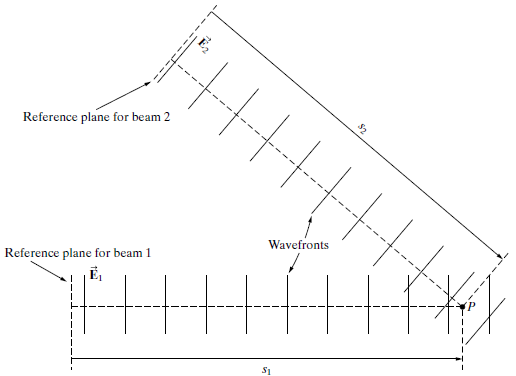
\includegraphics[scale=0.7]{Imagenes/Interferencia2_01.png}
    \caption{Interferencia de dos haces.}
    \label{fig:figura_07_01}
\end{figure}
Luego $\phi_{1}$ y $\phi_{2}$ representan las fases de estas ondas en sus respectivas fuentes en el tiempo $t = 0$. Estas ondas se combinan para producir una perturbación en el punto $P$, cuyo campo eléctrico $\va{E}_{p}$ está dado por el principio de superposición:
\begin{align*}
\va{E}_{p} = \va{E}_{1} + \va{E_{2}}
\end{align*}

Cabe señalar que $\va{E}_{1}$ y $\va{E_{2}}$ son funciones que varían rápidamente con frecuencias ópticas del orden de \num{d14} a \num{d15} \, \unit{\hertz} para la luz visible. Por tanto, ambos $\va{E}_{1}$ y $\va{E_{2}}$ promedian a cero en intervalos de tiempo muy cortos. La medición de las ondas por su efecto sobre el ojo o algún otro detector de luz depende de la energía del haz de luz. La densidad de potencia radiante, o \textit{irradiancia}, $E_{e} \, (\unit{\watt\per\square\meter})$ mide el promedio temporal del cuadrado de la amplitud de la onda. En la práctica, el promedio temporal lo realiza un detector. El tiempo promedio para el ojo es del orden de $1/30$ de segundo; otros detectores tienen tiempos promedio de tan solo un nanosegundo. En general, el tiempo promedio de los detectores físicos excede con creces el período óptico (\num{d-10} a \SI{d-15}{\second}).
\par
Desafortunadamente, el símbolo estándar para la irradiancia, excepto el subíndice, es el mismo que el del campo eléctrico. Para evitar confusiones, utilizamos aquí el símbolo $I$ para irradiancia, de modo que:
\begin{align}
I = \epsilon_{0} \, c \, \langle \va{E} \cdot \va{E} \rangle
\label{eq:ecuacion_07_03}
\end{align}
Por tanto, la irradiancia resultante en $P$ viene dada por:
\begin{align*}
I &= \epsilon_{0} \, c \, \expval{\va{E}_{p}^{2}} = \epsilon_{0} \, c \, \langle \va{E}_{p} \cdot \va{E}_{p} \rangle = \\
&= \epsilon_{0} \, c \, \expval{(\va{E}_{1} + \va{E}_{2}) \cdot (\va{E}_{1} + \va{E}_{2})}
\end{align*}
o equivalentemente
\begin{align}
I = \epsilon_{0} \, c \, \expval{ \va{E}_{1} \cdot \va{E}_{1} + \va{E}_{2} \cdot \va{E}_{2} + 2 \, \va{E}_{1} \cdot \va{E}_{2}}
\label{eq:ecuacion_07_04}
\end{align}
En la ecuación (\ref{eq:ecuacion_07_04}), los dos primeros términos corresponden a las irradiancias de las ondas individuales, $I_{1}$ e $I_{2}$. El último término depende de una interacción de las ondas y se llama \textit{término de interferencia} $I_{12}$. Entonces podemos escribir:
\begin{align}
I = I_{1} + I_{2} + I_{12}
\label{eq:ecuacion_07_05}
\end{align}

Si la luz se comportara sin interferencias, como las partículas clásicas, entonces esperaríamos que $I = I_{1} + I_{2}$. La presencia del tercer término $I_{12}$ es indicativo de la naturaleza ondulatoria de la luz, que puede producir un aumento o una disminución de la irradiancia a través de la interferencia. Observe que cuando $\va{E}_{1}$ y $\va{E}_{2}$ son ortogonales, de modo que su producto escalar desaparece, no se produce interferencia. Por el contrario, cuando los campos eléctricos son paralelos, el término de interferencia hace su máxima contribución. Dos haces de luz no polarizada producen interferencia porque cada uno se puede resolver en componentes ortogonales de $\va{E}$ que luego se pueden emparejar con componentes similares del otro haz. Cada componente produce un término de interferencia con $\va{E}_{1} \parallel \va{E}_{2}$ ($\va{E}_{1}$ paralelo a $\va{E}_{2}$).
\par
Consideremos el término de interferencia:
\begin{align}
I_{12} = 2 \, \epsilon_{0} \, c \, \expval{ \va{E}_{1} \cdot \va{E}_{2}}
\label{eq:ecuacion_07_06}
\end{align}
donde $\va{E}_{1}$ y $\va{E}_{2}$ están dados por las ecuaciones (\ref{eq:ecuacion_07_01}) y (\ref{eq:ecuacion_07_02}). Su producto punto:
\begin{align*}
\va{E}_{1} \cdot \va{E}_{2} = E_{01} \cdot E_{02} \, \cos (k \, s_{1} - \omega \, t + \phi_{1}) \, \cos (k \, s_{2} - \omega \, t + \phi_{2})
\end{align*}
se puede simplificar de manera instructiva usando una identidad trigonométrica. Para ello definamos
\begin{align*}
\alpha \equiv k \, s_{1} + \phi_{1} \hspace{0.2cm} \text{y} \hspace{0.2cm} \beta \equiv k \, s_{2} + \phi_{2}
\end{align*}
por lo que:
\begin{align*}
2 \, \va{E}_{1} \cdot \va{E}_{2} = 2 \, E_{01} \cdot E_{02} \, \cos(\alpha - \omega \, t) \, \cos(\beta - \omega \, t)
\end{align*}
La identidad:
\begin{align*}
2 \cos A \, \cos B = \cos (A + B) + \cos (B - A)
\end{align*}
nos ayudará a calcular el tiempo promedio de $2 \, \va{E}_{1} \cdot \va{E}_{2}$ como:
\begin{align*}
2 \, \expval{\va{E}_{1} \cdot \va{E}_{2}} = \va{E}_{01} \cdot \va{E}_{02} \left[ \expval{\cos (\alpha + \beta - 2 \omega \, t)} + \expval{\cos (\beta - \alpha)} \right]
\end{align*}
El primer promedio temporal en esta relación se toma sobre una función coseno que oscila rápidamente y por lo tanto es cero. De este modo:
\begin{align}
\begin{aligned}[b]
2 \, \expval{\va{E}_{1} \cdot \va{E}_{2}} &= \va{E}_{01} \cdot \va{E}_{02} \, \expval{\cos (\beta -\alpha)} = \\
&= \va{E}_{01} \cdot \va{E}_{02} \, \expval{ \cos(k (s_{2} - s_{1}) + \phi_{2} - \phi_{1})} = \\
&= \va{E}_{01} \cdot \va{E}_{02} \, \expval{\cos \delta}
\end{aligned}
\label{eq:ecuacion_07_07}
\end{align}
donde hemos definido la diferencia de fase entre $\va{E_{2}}$ y $\va{E}_{1}$ como:
\begin{align}
\delta = k \, (s_{2} - s_{1}) + \phi_{2} - \phi_{1}
\label{eq:ecuacion_07_08}
\end{align}

Para campos puramente monocromáticos, $\delta$ es independiente del tiempo, en cuyo caso $\expval{\cos \delta} = \cos \delta$. Sin embargo, como veremos, para campos reales, que no son perfectamente monocromáticos, se debe tener cuidado al tratar este promedio de tiempo. Combinando las ecuaciones (\ref{eq:ecuacion_07_06}) y (\ref{eq:ecuacion_07_07}):
\begin{align}
I_{12} = \epsilon_{0} \, c \, \va{E}_{01} \cdot \va{E}_{02} \, \expval{\cos \delta}
\label{eq:ecuacion_07_09}
\end{align}
Los términos de irradiancia $I_{1}$ e $I_{2}$ de la ecuación (\ref{eq:ecuacion_07_05}) se puede demostrar que produce:
\begin{align}
I_{1} = \epsilon_{0} \, c \, \expval{\va{E}_{1} \cdot \va{E}_{1}} = \epsilon_{0} \, c \, E_{01}^{2} \, \expval{\cos^{2} (\alpha - \omega \, t)} = \dfrac{1}{2} \epsilon_{0} \, c \, E_{01}^{2}
\label{eq:ecuacion_07_10}
\end{align}
y
\begin{align}
I_{2} = \epsilon_{0} \, c \, \expval{\va{E}_{2} \cdot \va{E}_{2}} = \epsilon_{0} \, c \, E_{02}^{2} \, \expval{\cos^{2} (\beta - \omega \, t)} = \dfrac{1}{2} \epsilon_{0} \, c \, E_{02}^{2}
\label{eq:ecuacion_07_11}
\end{align}
En las ecuaciones (\ref{eq:ecuacion_07_10}) y (\ref{eq:ecuacion_07_11}) utilizamos el hecho de que el promedio temporal del cuadrado de una función sinusoidal que oscila rápidamente es $1/2$. En la ecuación (\ref{eq:ecuacion_07_09}) cuando $E_{01} \parallel E_{02}$, su producto escalar es idéntico al producto de sus magnitudes $E_{01}$ y $E_{02}$. Estos pueden expresarse en términos de $I_{1}$ e $I_{2}$ mediante el uso de las Ecs. (\ref{eq:ecuacion_07_10}) y (\ref{eq:ecuacion_07_11}), y cuando se combina con la ecuación (\ref{eq:ecuacion_07_09}) da como resultado
\begin{align}
I_{12} = 2 \, \sqrt{I_{1} \, I_{2}} \, \expval{\cos \delta}
\label{eq:ecuacion_07_12}
\end{align}
y finalmente podemos escribir:
\begin{align}
I = I_{1} + I_{2} + 2 \, \sqrt{I_{1} \, I_{2}} \, \expval{\cos \delta}
\label{eq:ecuacion_07_13}
\end{align}

Observa que una vez que hemos asumido que los campos $\va{E}$ son paralelos, el tratamiento se vuelve muy similar al de la teoría escalar.

\section{Interferencia de campos mutuamente incoherentes.}

En la práctica, para campos eléctricos $\va{E}_{1}$ y $\va{E}_{2}$ provenientes de diferentes fuentes, el promedio de tiempo en la ecuación (\ref{eq:ecuacion_07_13}) es cero. Esto ocurre porque ninguna fuente es perfectamente monocromática. Para modelar fuentes reales, las Ecs. (\ref{eq:ecuacion_07_01}) y (\ref{eq:ecuacion_07_02}) deben modificarse para tener en cuenta las desviaciones de la monocromaticidad. Una forma de hacer esto es permitir que las fases $\phi_{1}$ y $\phi_{2}$ sean funciones del tiempo. Para las fuentes láser, estas fases normalmente serían funciones aleatorias del tiempo que varían en una escala de tiempo mucho más larga que un período óptico pero aún más corta que los tiempos promedio típicos del detector. El término de interferencia $I_{12}$ en este caso toma la forma:
\begin{align*}
2 \, \sqrt{I_{1} \, I_{2}} \, \expval{\cos(k (s_{2} - s_{1}) + \phi_{2} (t) - \phi_{1} (t))}
\end{align*}

Como se indicó, para detectores reales y para todas, excepto aquellas fuentes láser con estabilidad de frecuencia actualizada, el promedio de tiempo en la relación anterior será cero. En tal caso decimos que las fuentes son mutuamente incoherentes y la irradiancia detectada será:
\begin{align*}
I = I_{1} + I_{2} \hspace{1cm} \text{haces mutuamente incoherentes}
\end{align*}

Por lo tanto, a menudo se dice que los haces de luz procedentes de fuentes independientes, incluso si ambas fuentes son el mismo tipo de láser, no interfieren entre sí. De hecho, estos campos interfieren, pero el término de interferencia promedia cero durante los tiempos promedio de la mayoría de los detectores reales.

\section{Interferencia de haces mutuamente coherentes.}

Si la luz de la misma fuente láser se divide y luego se recombina en un detector, el tiempo promedio en la ecuación (\ref{eq:ecuacion_07_13}) no tiene por qué ser cero. Esto ocurre porque las desviaciones de la monocromaticidad de cada haz, aunque sigan presentes, estarán correlacionadas ya que ambos haces provienen de la misma fuente. En este caso, la diferencia de fase $\phi_{2} (t) - \phi_{1} (t)$ será estrictamente cero si los haces recorren trayectorias de \textit{igual duración} antes de recombinarse en el detector. En tal caso, $\delta$ es una constante y el término de interferencia toma la forma:
\begin{align*}
2 \, \sqrt{I_{1} \, I_{2}} \, \expval{\cos(k (s_{2} - s_{1}) + \phi_{1} (t) - \phi_{1} (t))} &= 2 \, \sqrt{I_{1} \, I_{2}} \, \cos(k (s_{2} - s_{1})) \\
&= 2 \, \sqrt{I_{1} \, I_{2}} \, \cos \delta
\end{align*}

Incluso si los campos eléctricos recorren trayectorias que difieren en duración en un tiempo $\delta t$, la diferencia de fase resultante de la salida de la monocromaticidad $\phi_{1} (t) - \phi_{1} (t - \delta t)$, seguirá siendo casi cero mientras $\delta_{t}$ sea menor que el llamado \textit{tiempo de coherencia} $\tau_{0}$ de la fuente. Cualitativamente, el tiempo de coherencia de la fuente es el intervalo de tiempo durante el cual se producen desviaciones de la monocromaticidad son pequeños. Aprenderemos que el tiempo de coherencia de una fuente es inversamente proporcional al rango de frecuencias $\Delta \nu$, de los componentes que componen el campo eléctrico. Eso es:
\begin{align*}
\tau_{0} = \dfrac{1}{\Delta \nu}
\end{align*}

Asociado con el tiempo de coherencia de una fuente está la longitud de coherencia, $l_{t} = c \, \tau_{0}$, que es la distancia que recorre el campo eléctrico en un tiempo de coherencia. Para una fuente de luz blanca, la longitud de coherencia es aproximadamente \SI{1}{\micro\meter}. Las fuentes láser tienen longitudes de coherencia que varían desde decenas de centímetros hasta decenas de kilómetros. A lo largo del resto de este tema, supondremos que la diferencia en las longitudes de los caminos recorridos por los haces que se originan en la misma fuente es considerablemente menor que la longitud de coherencia de la fuente. En tal caso, se dice que los campos eléctricos son mutuamente coherentes y la irradiancia de los campos combinados tendrá la forma:
\begin{align}
I = I_{1} + I_{2} + 2 \, \sqrt{I_{1} \, I_{2}} \, \cos \delta \hspace{1cm} \text{Haces mutuamente coherentes}
\label{eq:ecuacion_07_14}
\end{align}
donde $\delta$ es la diferencia de fase total en el punto de recombinación del haz. Como hemos observado, si los haces se originan en la misma fuente, esta diferencia de fase se acumula como resultado de una diferencia en las longitudes de trayectoria recorridas por los respectivos haces. En muchos casos de interés, otros factores también pueden provocar una diferencia de fase entre los haces. Mecanismos importantes de este tipo incluyen diferentes cambios de fase debido a la reflexión de los divisores de haz y diferentes índices de refracción en las trayectorias separadas tomadas por los dos haces. Dependiendo de si $\cos \delta > 0$ o $\cos \delta < 0$ en la ec. (\ref{eq:ecuacion_07_14}), el término de interferencia aumenta o disminuye la suma de las irradiancias individuales $I_{1}$ e $I_{2}$, conduce a una interferencia constructiva o destructiva, respectivamente. Dado que las distancias relativas recorridas por los dos haces diferirán, en general, para diferentes puntos de observación en la región de superposición, la diferencia de fase $\delta$ también será diferente para diferentes puntos de observación. Normalmente, $\cos \delta$ adoptará valores máximos y mínimos alternos y en el plano de observación aparecerán \textit{franjas de interferencia}, separadas espacialmente.
\par
Para ser más específicos, cuando $\cos \delta = +1$ la interferencia constructiva produce la máxima irradiancia:
\begin{align}
I_{\max} = I_{1} + I_{2} + 2 \, \sqrt{I_{1} \, I_{2}}
\label{eq:ecuacion_07_15}
\end{align}
Esta condición ocurre siempre que la diferencia de fase $\delta = 2 m \pi$, donde $m$ es cualquier número entero o cero. Por otra parte, cuando $\cos \delta = -1$ la interferencia destructiva produce la irradiancia mínima, o de fondo:
\begin{align}
I_{\min} = I_{1} + I_{2} - 2 \, \sqrt{I_{1} \, I_{2}}
\label{eq:ecuacion_07_16}
\end{align}
una condición que ocurre siempre $\delta = (2 m + 1) \pi$. Una gráfica de irradiancia $I$ versus fase $\delta$, en la figura (\ref{fig:figura_07_02a})  muestra franjas periódicas.
\begin{figure}[H]
    \centering
    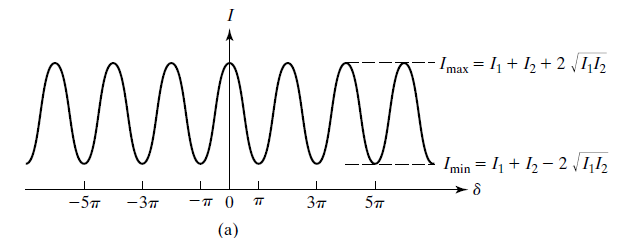
\includegraphics[scale=0.8]{Imagenes/Interferencia2_02a.png}
    \caption{Irradiación de franjas de interferencia en función de la diferencia de fase.}
    \label{fig:figura_07_02a}
\end{figure}
La interferencia destructiva es completa, es decir, la cancelación es completa, cuando $I_{1} = I_{2} = I_{0}$. Entonces, las Ecs. (\ref{eq:ecuacion_07_15}) y (\ref{eq:ecuacion_07_16}) dan:
\begin{align*}
I_{\max} = 4 \, I_{0} \hspace{0.2cm} \text{y} \hspace{0.2cm} I_{\min} = 0
\end{align*}
\begin{figure}[H]
    \centering
    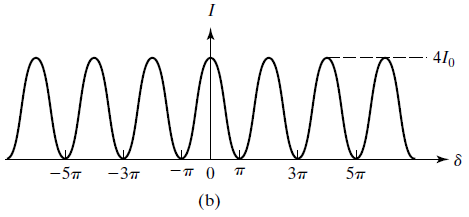
\includegraphics[scale=0.8]{Imagenes/Interferencia2_02b.png}
    \caption{La visibilidad aumenta en (b), donde la irradiancia de fondo $I_{\min} = 0$ cuando $I_{1} = I_{2}$.}
    \label{fig:figura_07_02b}
\end{figure}
Las franjas resultantes, que se muestran en la figura (\ref{fig:figura_07_02b}), ahora muestran un mejor contraste. Una medida de \textit{contraste marginal}, llamada \textit{visibilidad}, con valores entre 0 y 1, viene dada por la cantidad:
\begin{align}
\text{visibilidad} = \dfrac{I_{\max} - I_{\min}}{I_{\max} + I_{\min}}
\label{eq:ecuacion_07_17}
\end{align}
Por lo tanto, en el uso experimental de patrones marginales, normalmente es deseable garantizar que los haces perturbadores tengan las mismas amplitudes.

Otra forma útil de la ecuación (\ref{eq:ecuacion_07_14}), para el caso de haces de igual amplitud que interfieran, de manera que $I_{1} = I_{2} = I_{0}$, se encuentra escribiendo:
\begin{align*}
I = I_{0} + I_{0} + 2 \, \sqrt{I_{0}^{2}} \, \cos \delta = 2 \, I_{0} \left( 1 + \cos \delta \right)
\end{align*}
que al usar la siguiente identidad trigonométrica:
\begin{align*}
1 + \cos \delta \equiv 2 \, \cos^{2} \left( \dfrac{\delta}{2} \right)
\end{align*}
La irradiancia de dos haces iguales interfiriendo, es entonces:
\begin{align}
I = 4 \, I_{0} \, \cos^{2} \left( \dfrac{\delta}{2} \right)
\label{eq:ecuacion_07_18}
\end{align}
Observa que la energía no se conserva en cada punto de la superposición, es decir, $I \neq 2 \, I_{0}$ sino que durante al menos un período espacial del patrón marginal $I_{\text{av}} = 2 \, I_{0}$. Esta situación es típica de los fenómenos de interferencia y difracción: si la densidad de potencia cae por debajo de la media en algunos puntos, en otros aumenta por encima de la media, de tal manera que el patrón total satisface el principio de conservación de energía.

\vspace{0.5cm}
\noindent
\textbf{Ejemplo 1:} Consideremos dos haces de interferencia con campos eléctricos paralelos que están superpuestos. Toma los campos eléctricos de los haces individuales como:
\begin{align*}
E_{1} &= 2 \, \cos \left( k \, s_{1} - \omega \, t \right) \hspace{0.3cm} (\unit{\kilo\volt\per\metre}) \\[0.5em]
E_{2} &= 5 \, \cos \left( k \, s_{2} - \omega \, t \right) \hspace{0.3cm} (\unit{\kilo\volt\per\metre})
\end{align*}
\noindent
\textbf{Solución:}
Determinemos la irradiancia aportada por cada haz actuando solo y debido a su interferencia mutua en un punto donde su diferencia de trayectoria es tal que:
\begin{align*}
k \left( s_{2} - s_{1} \right) = \pi / 12
\end{align*}
tenemos entonces que:
\begin{align*}
I_{1} &= \dfrac{1}{2} \epsilon_{0} \, c \, E_{01}^{2} = \dfrac{1}{2} \epsilon_{0} \, c \left( 2000 \right)^{2} = \SI{5309}{\watt\per\square\meter} \\[0.5em]
I_{2} &= \dfrac{1}{2} \epsilon_{0} \, c \, E_{02}^{2} = \dfrac{1}{2} \epsilon_{0} \, c \left( 5000 \right)^{2} = \SI{33180}{\watt\per\square\meter} \\[0.5em]
I_{12} &= 2 \, \sqrt{I_{1} \, I_{2}} \, \cos \delta = 2 \, \sqrt{(5309 \cdot 33180)} \, \cos (\pi/12) = \SI{25640}{\watt\per\square\meter}
\end{align*}
Para obtener la visibilidad cercana a este punt de recombinación, debemos de calcular:
\begin{align*}
I_{\max} &= I_{1} + I_{2} + 2 \, \sqrt{I_{1} \, I_{2}} = 5309 + 33180 + 2 \sqrt{(5309 \cdot 33180)} =  \SI{65034}{\watt\per\square\meter} \\[0.5em]
I_{\min} &= I_{1} + I_{2} - 2 \, \sqrt{I_{1} \, I_{2}} = 5309 + 33180 - 2 \sqrt{(5309 \cdot 33180)} =  \SI{11945}{\watt\per\square\meter}
\end{align*}
La visibilidad se definió por la ecuación (\ref{eq:ecuacion_07_17}), así que:
\begin{align*}
\text{visibilidad} = \dfrac{65034 - 11945}{65304 + 11945} = 0.690
\end{align*}
Si las amplitudes de las dos ondas son iguales, entonces $I_{\max} = 4 \, I_{0}$, junto con $I_{\min} = 0$, y la visibilidad sería igual a $1$.

En el análisis que conduce a la irradiancia que resulta de la superposición de dos haces mutuamente coherentes, la ec. (\ref{eq:ecuacion_07_14}), asumimos que los haces individuales eran ondas planas descritas por las ecs. (\ref{eq:ecuacion_07_01}) y (\ref{eq:ecuacion_07_02}). De hecho, el análisis es válido para cualquier tipo de onda armónica (por ejemplo, esférica, cilíndrica o Gaussiana). Sin embargo, para este tipo de ondas, las amplitudes $E_{01}$ y $E_{02}$ (y por tanto las irradiancias $I_{1}$ e $I_{2}$) dependen de la distancia desde la fuente al punto de observación.

\section{El experimento de doble rendija de Young.}

El experimento decisivo realizado por Thomas Young en 1802 se muestra esquemáticamente en la figura (\ref{fig:figura_07_03}).
\begin{figure}[H]
    \centering
    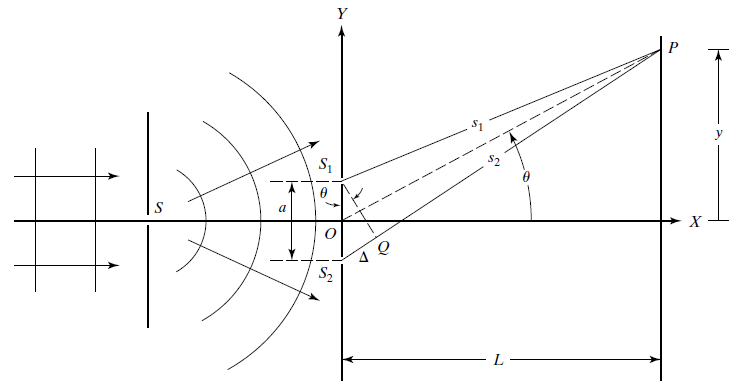
\includegraphics[scale=0.8]{Imagenes/Interferencia2_03.png}
    \caption{Esquema del experimento de la doble rendija de Young. Los agujeros $S_{1}$ y $S_{2}$ suelen ser hendiduras y las dimensiones largas se extienden hacia la página. El agujero en $S$ no es necesario si la fuente es un láser espacialmente coherente.}
    \label{fig:figura_07_03}
\end{figure}

Primero se deja pasar luz monocromática a través de un pequeño orificio para aproximarse a una única fuente puntual $S$. La luz se propaga en ondas esféricas desde la fuente $S$ de acuerdo con según el principio de Huygens y se le permite caer sobre un plano con dos agujeros muy próximos entre sí, $S_{1}$ y $S_{2}$. En una versión moderna de este experimento, normalmente se utiliza un láser para iluminar los dos agujeros. En cualquier caso, los agujeros se convierten en dos fuentes de luz coherentes, cuya interferencia se puede observar en una pantalla a cierta distancia. Si los dos agujeros son iguales en tamaño, las ondas de luz que emanan de los agujeros tienen amplitudes comparables, y la irradiancia en cualquier punto de superposición viene dada por la ecuación (\ref{eq:ecuacion_07_18}).
\par
Con referencia a la figura (\ref{fig:figura_07_03}), ahora desarrollaremos una expresión para la irradiancia en puntos de observación como $P$ en una pantalla que está a una distancia $L$ del plano que contiene los dos agujeros $S_{1}$ y $S_{2}$. La diferencia de fase $\delta$ entre las dos ondas que llegan al punto de observación $P$ debe determinarse para calcular la irradiancia resultante allí. Claramente, si:
\begin{align*}
S_{2} \, P - S_{1} \, P = s_{2} - s_{2} = m \, \lambda
\end{align*}
las ondas llegarán en fase, se obtendrá la máxima irradiancia o brillo. Si se cumple la condición:
\begin{align*}
s_{2} - s{1} = \left( m + \dfrac{1}{2} \right) \, \lambda
\end{align*}
requerida para una interferencia destructiva u oscuridad. En términos prácticos, la separación de los agujeros $a$ es mucho menor que la distancia de la pantalla $L$, lo que permite una expresión simple para la distancia del camino $s_{2} - s_{1}$. Usando $P$ como centro, dibuje un arco $S_{1} \, Q$ de radio $s_{1}$ de modo que interseque la línea $S_{2} \, P$ en $Q$. Entonces $s_{2} - s_{1}$ es igual al segmento $\Delta$, como se muestra. La primera aproximación es considerar el arco $S_{1} \, Q$ como un segmento de línea recta que forma un cateto del triángulo rectángulo $S_{1} \, S_{2} \,Q$. Si $\theta$ es el ángulo entre los segmentos de línea $S_{1} \, S_{2}$ y $S_{1} \, Q$, entonces $\Delta = a \, \sin \theta$. La segunda aproximación identifica el ángulo $\theta$ con el ángulo entre el eje óptico $OX$ y la línea trazada desde el punto medio $O$ entre los agujeros hasta el punto $P$ en la pantalla. Observa que los lados correspondientes de los dos ángulos $\theta$ están relacionados de manera que $O \, X \perp S_{1} \, S_{2}$ y $OP$ es casi exactamente perpendicular a $S_{1} \, Q$.
\par
La condición para la \textit{interferencia constructiva} en un punto $P$ de la pantalla es, entonces, una muy buena aproximación:
\begin{align}
s_{2} - s_{1} = \Delta = m \, \lambda \cong a \, \sin \theta
\label{eq:ecuacion_07_19}
\end{align}
mientras que para una \textit{interferencia destructiva}:
\begin{align}
\Delta = \left( m + \dfrac{1}{2} \right) \, \lambda \cong a \, \sin \theta
\label{eq:ecuacion_07_20}
\end{align}
donde $m$ es cero o un valor entero. Normalmente, en los puntos de observación de interés, las \textit{amplitudes} del campo eléctrico de los haces que se originan en las dos rendijas son casi iguales, de modo que la irradiancia en la pantalla, en un punto determinado por el ángulo $\theta$, se encuentra utilizando la ecuación (\ref{eq:ecuacion_07_18}) y la relación entre la diferencia de trayectoria $\Delta$ y la diferencia de fase $\delta$:
\begin{align*}
\delta = k \left( s_{2} - s_{1} \right) = \dfrac{2 \pi}{\lambda} \, \Delta
\end{align*}
El resultado es:
\begin{align*}
I = 4 \, I_{0} \, \cos^{2} \left( \dfrac{\pi \, \Delta}{\lambda} \right) = 4 \, I_{0} \, \cos^{2} \left( \dfrac{\pi \, a \, \sin \theta}{\lambda} \right)
\end{align*}
Para puntos $P$ cercanos al eje óptico, donde $y \ll L$ podemos aproximarnos más para que:
\begin{align*}
\sin \theta \cong \tan \theta \cong \dfrac{y}{L}
\end{align*}
así que:
\begin{align*}
I = 4 \, I_{0} \, \cos^{2} \left( \dfrac{\pi \, a \, y}{\lambda \, L} \right)
\label{eq:ecuacion_07_21}
\end{align*}
Al permitir la función coseno en la ecuación (\ref{eq:ecuacion_07_21}) para convertirse alternativamente en  $\pm 1$ y $0$, se producen las condiciones expresadas por las ecs.  (\ref{eq:ecuacion_07_19}) y (\ref{eq:ecuacion_07_21}) para interferencia constructiva y destructiva.
\par
Argumentando ahora a partir de la ec. (\ref{eq:ecuacion_07_19}) y la relación de ángulo pequeño
\begin{align*}
\sin \theta \cong \tan \theta \cong \dfrac{y}{L}
\end{align*}
encontramos que las posiciones de las franjas brillantes están dadas por:
\begin{align}
y_{m} = \dfrac{m \, \lambda \, L}{a} \hspace{1cm} m = 0, \pm 1, \pm 2, \ldots
\end{align}

En consecuencia, existe una separación constante entre los máximos de irradiancia, correspondientes a valores sucesivos de $m$, dados por:
\begin{align}
\Delta  y = y_{m+1} - y_{m} = \dfrac{\lambda \, L}{a}
\label{eq:ecuacion_07_23}
\end{align}
con mínimos situados a medio camino entre los máximos. Por lo tanto, la separación de franjas es proporcional tanto a la longitud de onda como a la distancia de la pantalla e inversamente proporcional al espaciado de los agujeros. Al reducir el espacio entre los agujeros se amplía el patrón de flecos formado por cada color. La medición de la separación de franjas proporciona un medio para determinar la longitud de onda de la luz. El orificio único, utilizado para asegurar cierto grado de coherencia espacial, puede eliminarse si se utiliza luz láser, altamente monocromática y espacialmente coherente, para iluminar la doble rendija. En la disposición de observación que se acaba de describir, las franjas se observan en una pantalla colocada perpendicular al eje óptico a cierta distancia de la apertura, como se indica en la figura (\ref{fig:figura_07_04}).
\begin{figure}[H]
    \centering
    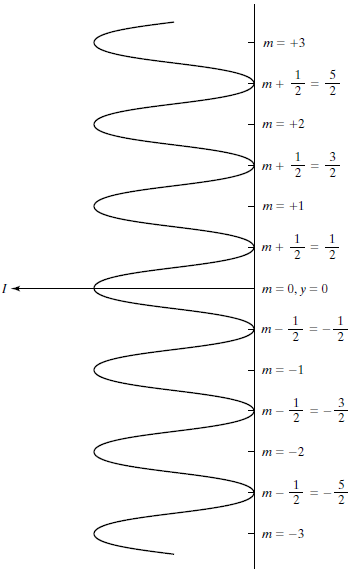
\includegraphics[scale=0.8]{Imagenes/Interferencia2_04.png}
    \caption{Irradiancia versus distancia desde el eje óptico para un patrón de franjas de doble rendija. El orden del patrón de interferencia está indicado por $m$, y los valores integrales de m determinan las posiciones de los máximos marginales.}
    \label{fig:figura_07_04}
\end{figure}
Los máximos de las franjas coinciden con órdenes integrales de $m$, y los mínimos de las franjas caen a mitad de camino entre los máximos adyacentes.
\par
\noindent
\textbf{Ejemplo 2:} La luz láser pasa a través de dos rendijas idénticas y paralelas, separadas por \SI{0.2}{\milli\meter}. Se ven franjas de interferencia en una pantalla a \SI{1}{\meter} de distancia Los máximos de interferencia están separados por \SI{3.29}{\milli\meter}. ¿Cuál es la longitud de onda de la luz? ¿Cómo varía la irradiancia en la pantalla, si la contribución de una sola rendija es $I_{0}$?

\noindent
\textbf{Solución:} De la ec. (\ref{eq:ecuacion_07_23}):
\begin{align*}
\lambda &= \dfrac{a \, \Delta y}{L} = \dfrac{(\SI{0.0002}{\meter})(\SI{3.29d-3}{\meter})}{\SI{1}{\meter}} = \\[0.5em]
&= \SI{6.58d-7}{\meter} = \SI{658}{\nano\meter}
\end{align*}
En conformidad con la ec. (\ref{eq:ecuacion_07_21}): $I = 4 \, I_{0} \, \cos^{2} \left[ \dfrac{\pi \,a \, y}{\lambda \, L} \right]$. En este caso:
\begin{align*}
I = 4 \, I_{0} \, \cos^{2} \left[ \dfrac{\pi (0.0002) y}{(\num{658d-9}(\SI{1}{\meter}))} \right] = 4 \, I_{0} \, \cos^{2} \left[ (955) y \right]
\end{align*}

En la figura (\ref{fig:figura_07_05}) se muestra una forma alternativa de ver la formación de posiciones brillantes $(B)$ de interferencia constructiva y posiciones oscuras $(D)$ de interferencia destructiva.
\begin{figure}[H]
    \centering
    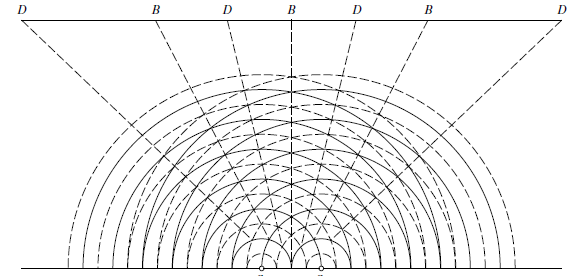
\includegraphics[scale=0.8]{Imagenes/Interferencia2_05.png}
    \caption{La luz procedente de dos fuentes coherentes produce franjas de interferencia alternas brillantes y oscuras. A lo largo de las direcciones donde se obtienen las crestas (círculos sólidos) de $S_{1}$ las crestas de intersección de $S_{2}$, resulta el brillo $(B)$. A lo largo de las direcciones donde las crestas se encuentran con los valles (círculos discontinuos), se produce oscuridad $(D)$.}
    \label{fig:figura_07_05}
\end{figure}
Las crestas y valles de ondas esféricas desde $S_{1}$ y $S_{2}$ acercándose a la pantalla. A lo largo de las direcciones marcadas con $B$, las crestas de las ondas (o valles de las ondas) de ambas rendijas coinciden, produciendo la máxima irradiancia. Por otro lado, a lo largo de las direcciones marcadas con $D$, se ve que las ondas están desfasadas en media longitud de onda, lo que produce interferencias destructivas.
\par
Obviamente, deben estar presentes franjas en todo el espacio que rodea los agujeros, donde se permite que la luz de los agujeros interfiera, aunque la irradiancia es mayor en la dirección de avance. Si imaginamos dos fuentes puntuales coherentes de luz irradiando en todas direcciones, entonces la condición dada por la ecuación. (19) para franjas brillantes:
\begin{align}
s_{2} - s_{1} = m \, \lambda
\label{eq:ecuacion_07_24}
\end{align}
define una familia de superficies de franjas brillantes en el espacio que rodea los agujeros. Para visualizar este conjunto de superficies, podemos aprovechar la simetría inherente a la disposición. En la figura (\ref{fig:figura_07_06}), se muestra la intersección de varias superficies de franjas brillantes con un plano que incluye las dos fuentes, correspondiendo cada superficie a un valor entero de orden $m$.
\begin{figure}[H]
    \centering
    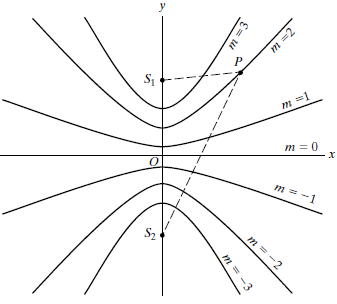
\includegraphics[scale=0.8]{Imagenes/Interferencia2_06.png}
    \caption{Superficies de franjas brillantes para dos fuentes puntuales coherentes. Las distancias desde $S_{1}$ y $S_{2}$ hacia cualquier punto $P$ en una superficie de franja brillante difieren en un número entero de longitudes de onda. Las superficies se generan girando el patrón alrededor del eje y.}
    \label{fig:figura_07_06}
\end{figure}
Las superficies son hiperbólicas, ya que la ec. (24) es precisamente la condición para una familia de curvas hiperbólicas con parámetro $m$. En la medida que el eje $y$ es un eje de simetría, las superficies de franja brillantes correspondientes se generan girando todo el patrón alrededor del eje $y$. Entonces deberíamos poder visualizar la intersección de estas superficies con el plano de una pantalla de observación colocada en cualquier lugar cercano. En particular, una pantalla colocada perpendicular al eje $OX$, como en la figura (\ref{fig:figura_07_03}), intercepta arcos hiperbólicos que aparecen como franjas rectas cerca del eje, mientras que una pantalla colocada perpendicular al eje $OY$ muestra franjas circulares concéntricas centradas en el eje. Debido a que el sistema de franjas se extiende por todo el espacio que rodea las dos fuentes, se dice que las franjas \textit{no están localizadas}.
\par
Los orificios $S$, $S_{1}$ y $S_{2}$ de la figura (\ref{fig:figura_07_03}) generalmente se reemplazan por hendiduras estrechas y paralelas (orientadas con sus lados largos perpendiculares a la página en la figura \ref{fig:figura_07_03}) para iluminar más completamente el patrón de interferencia. El efecto del conjunto de fuentes puntuales a lo largo de las rendijas, cada conjunto produciendo su propio sistema de franjas como se acaba de describir, es simplemente alargar el patrón paralelo a las franjas, sin cambiar sus relaciones geométricas. Esto es cierto incluso cuando dos puntos a lo largo de una rendija fuente no son mutuamente coherentes.

\section{Interferencia en películas dieléctricas.}

La apariencia familiar de los colores en la superficie de las películas de agua aceitosa y jabón, las plumas de pavo real y las alas de las mariposas están asociadas con la interferencia de la luz en una o múltiples capas superficiales delgadas de material transparente. Existe una variedad de situaciones en las que puede tener lugar dicha interferencia, lo que afecta la naturaleza del patrón de interferencia y las condiciones bajo las cuales puede observarse. Las variables de la situación incluyen el tamaño y el ancho espectral de la fuente y la forma y reflectancia de la película. 
\par
Consideremos el caso de una película de material transparente delimitada por planos paralelos, como los que podrían formarse por una mancha de petróleo, una capa de óxido metálico o una capa evaporada sobre un sustrato de vidrio plano (figura \ref{fig:figura_07_10}).
\begin{figure}[H]
    \centering
    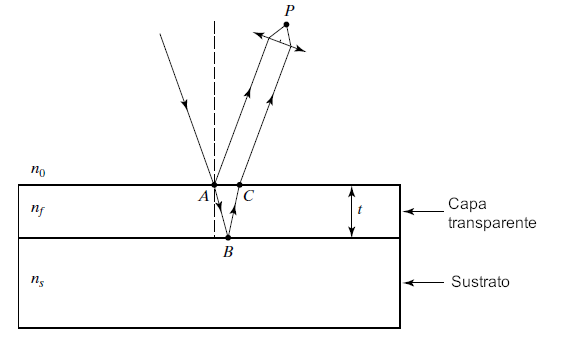
\includegraphics[scale=0.8]{Imagenes/Interferencia2_07.png}
    \caption{Interferencia de doble haz de una película. Los rayos reflejados desde las superficies planas superior e inferior de la película se juntan en $P$ mediante una lente.}
    \label{fig:figura_07_10}
\end{figure}
Un haz de luz que incide sobre la superficie de la película en $A$ se divide en porciones reflejadas y refractadas. Esta separación de la luz original en dos partes, previa a la recombinación y la interferencia, suele denominarse \textit{división de amplitud}, en contraste a una situación como la doble rendija de Young, en la que se dice que la separación se produce por \textit{división del frente de onda}. El haz refractado se refleja nuevamente en la interfaz película-sustrato $B$ y abandona la película en $C$, en la misma dirección que el haz reflejado en $A$. Parte del haz puede reflejarse internamente nuevamente en $C$ y continuar experimentando múltiples reflejos dentro de la capa de película, hasta que haya perdido su irradiancia. Por lo tanto, existirán múltiples haces paralelos que emergerán de la superficie superior, aunque con amplitudes que disminuyen rápidamente. A menos que la reflectancia de la película sea grande, una buena aproximación a la situación más compleja de reflexión múltiple es considerar sólo los dos primeros haces emergentes. Los dos haces paralelos que salen de la película en $A$ y $C$ pueden juntarse mediante una lente convergente, el ojo, por ejemplo. Los dos haces que se cruzan en $P$ se superponen e interfieren. Dado que los dos haces recorren caminos diferentes desde el punto $A$ en adelante, se desarrolla una diferencia de fase relativa que puede producir interferencia constructiva o destructiva en $P$. La diferencia de camino óptico $\Delta$, en el caso de incidencia normal, es la longitud de camino adicional $ABC$ recorrida por el índice de refracción de la película. De este modo:
\begin{align}
\Delta = n (A \, B + B \, C) = n (2 \, t)
\label{eq:ecuacion_07_26}
\end{align}
donde $t$ es el espesor de la película. Por ejemplo, si $2 \, n  \, t = \lambda_{0}$, la longitud de onda de la luz en el vacío, los dos haces que interfieren, basándose únicamente en la diferencia de trayectoria óptica, estarían en fase y producirían una interferencia constructiva. Sin embargo, se debe considerar una diferencia de fase adicional, debido al fenómeno de cambios de fase en la reflexión. Supongamos que $n_{f} > n_{0}$ y $n_{f} > n_{s}$. De hecho, a menudo $n_{0} = n_{s}$ porque los medios que rodean la película son idénticos, como en el caso de una película de agua (burbuja de jabón) en el aire. Entonces, la reflexión en $A$ ocurre con la luz que va desde un índice más bajo $n_{0}$ hasta un índice más alto $n_{f}$, una condición generalmente llamada \textit{reflexión externa}. La reflexión en $B$, por otro lado, ocurre cuando la luz pasa de un índice más alto $n-{f}$ a un índice más bajo $n_{s}$, una condición llamada \textit{reflexión interna}. Se produce un desplazamiento de fase relativo de $\pi$ entre los haces reflejados externa e internamente, de modo que, de manera equivalente, se introduce una diferencia de trayectoria adicional de $\lambda/2$ entre los dos haces. La diferencia neta de trayectoria óptica entre los haces es entonces $\lambda + \lambda/2$ lo que los desfasa precisamente y se produce una interferencia destructiva en $P$. Si, en cambio, ambas reflexiones son externas $(n_{0} < n_{f} < n_{s})$ o si ambas reflexiones son internas $(n_{0} > n_{f} > n_{s})$, no es necesario tomar en cuenta la diferencia de fase relativa debida a la reflexión. en cuenta. En ese caso, se produce interferencia constructiva en $P$.
\par
Un uso frecuente de tales películas monocapa es en la producción de \textit{recubrimientos antirreflectantes} sobre superficies ópticas. En la mayoría de los casos, la luz llega a la película desde el aire, de modo que $n_{0} =1$, además, si $n_{s} > n_{f}$ no se produce ningún cambio de fase relativo entre los dos haces reflejados, la diferencia en el camino óptico determina por sí sola el tipo de interferencia que se puede esperar. Si el espesor de la película es $\lambda_{f}/4$ donde $\lambda_{f}$ es la longitud de onda de la luz en la película, entonces $2 \, t = \lambda_{f}/2$ y la diferencia de trayectoria óptica $2 \, n_{f} \, t = \lambda_{0}/2$, ya que $\lambda_{0} = n_{f} \, \lambda_{f}$. Se produce interferencia destructiva en esta longitud de onda y, hasta cierto punto, en longitudes de onda vecinas, lo que significa que la luz reflejada por dicha película es la espectro incidente menos la región de longitud de onda alrededor $\lambda_{0}$. Si la luz incidente es blanca y $\lambda_{0}$ está en la región visible, la luz reflejada es de color. La extinción de una región del espectro mediante películas de $\lambda/4$ de espesor no reflectantes es, por supuesto, más eficaz si las amplitudes de los dos haces reflejados son iguales. En general, todo lo que se puede decir es que para la interferencia constructiva las dos amplitudes se suman (estando en fase), y para la interferencia destructiva las amplitudes se restan (estando exactamente desfasadas). Para que la diferencia sea cero, es decir, que la interferencia destructiva sea completa, las amplitudes deben ser iguales. En el caso de incidencia normal, el \textit{coeficiente de reflexión} (o relación entre las amplitudes del campo eléctrico reflejado e incidente) viene dado por:
\begin{align}
r = \dfrac{1 - n}{1 + n}
\label{eq:ecuacion_07_27}
\end{align}
donde el \textit{índice relativo} $n = n_{2}/n_{1}$. Las amplitudes del campo eléctrico reflejado interna y externamente desde la película de la figura (\ref{fig:figura_07_10}) son entonces iguales, suponiendo una película no absorbente, si los índices relativos son equivalentes para estos casos, es decir, si:
\begin{align}
\dfrac{n_{f}}{n_{0}} = \dfrac{n_{s}}{n_{f}} \hspace{1cm} \text{o} \hspace{1cm} n_{f} = \sqrt{n_{0} \, n_{s}}
\label{eq:ecuacion_07_28}
\end{align}

Ya que normalmente $n_{0} = 1$, el requisito de que los haces reflejados sean de igual amplitud se cumple eligiendo una película cuyo índice de refracción sea la raíz cuadrada del índice de refracción del sustrato. Puede que exista o no un material de película adecuado para la aplicación, y se llega a algún acuerdo. Por ejemplo, para reducir la reflectancia de las lentes empleadas en instrumentos ópticos que manejan luz blanca, el espesor de la película $\lambda/4$ se determina con una $\lambda$ en el centro del espectro visible o donde el sistema de detección sea más sensible. En el caso del ojo, esta es la porción de color amarillo verdoso cerca de los \SI{550}{\nano\meter}. Suponiendo que $n = 1.50$ para la lente de vidrio, idealmente $n_{f} = \sqrt{1.50} = 1.22$. El material de película práctico más cercano con un índice coincidente es $\text{MgF}_{2}$ con $n = 1.38$. Para un recubrimiento antirreflectante de este tipo, la luz reflejada reducida cerca de la mitad del espectro da como resultado un predominio de los extremos azul y rojo del espectro, de modo que los recubrimientos aparezcan de color púrpura con la luz reflejada.
\par
Como otro ejemplo, considera una pila multicapa de películas dieléctricas de índice alto y bajo alternadas (figura ).
\begin{figure}[H]
    \centering
    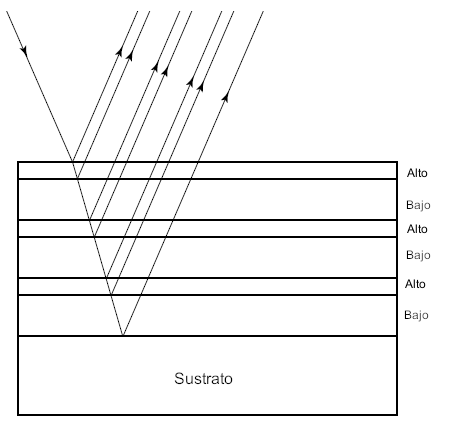
\includegraphics[scale=0.8]{Imagenes/Interferencia2_08.png}
    \caption{Espejo dieléctrico multicapa con índice alto y bajo alterno. Cada película tiene un espesor óptico de $\lambda > 4$.}
    \label{fig:figura_07_11}
\end{figure}
Si cada película tiene un espesor óptico de $\lambda_{f}/4$ un pequeño análisis se ve que en este caso todos los haces que emergen están en fase. Múltiples reflexiones en la región de $\lambda_{0}$ aumentan la intensidad total reflejada y la pila de cuarto de onda actúa como un espejo eficiente. Tales pilas multicapa pueden diseñarse para satisfacer la extinción o mejora de la luz reflejada en una porción mayor del espectro que lo haría una película de una sola capa.
\par
Volviendo ahora a la película de una sola capa, primero queremos generalizar las condiciones para la interferencia constructiva y destructiva calculando la diferencia de trayectoria óptica en el caso de que los rayos incidentes \textit{no sean normales}. La figura (\ref{fig:figura_07_12}) ilustra un rayo incidente sobre una película en un ángulo $\theta_{i}$.
\begin{figure}[H]
    \centering
    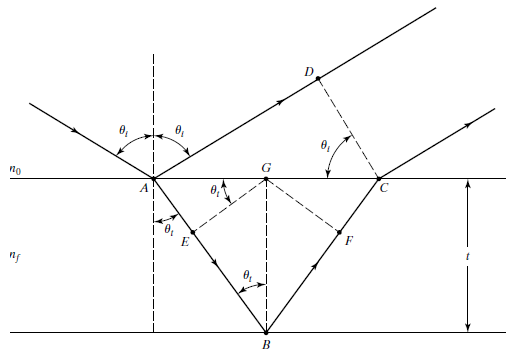
\includegraphics[scale=0.8]{Imagenes/Interferencia2_09.png}
    \caption{Interferencia de una sola película con luz incidente en un ángulo arbitrario $\theta_{i}$.}
    \label{fig:figura_07_12}
\end{figure}
La diferencia de fase en los puntos $C$ y $D$ entre haces emergentes se debe a la diferencia de trayectoria óptica entre las trayectorias $AD$ y $ABC$. Después de alcanzar los puntos $C$ y $D$, los respectivos haces son paralelos y en el mismo medio, de modo que no hay más diferencias de fase ocurre. Para ayudar en el cálculo, el punto $G$ se muestra a medio camino entre $A$ y $C$ al pie de la altitud $BG$ en el triángulo isósceles $ABC$. Los puntos $E$ y $F$ se determinan construyendo las perpendiculares $GE$ y $GF$ a las trayectorias de los rayos $AB$ y $BC$, respectivamente. La diferencia de trayectoria óptica entre los haces emergentes es, entonces:
\begin{align*}
\Delta = n_{f} (AB + BC) - n_{0} (AD)
\end{align*}
donde $n_{f}$ y $n_{0}$ son los índices de la película y el medio externo como se muestra.
\par
Es útil dividir las distancias $AB$ y $BC$ en partes y reorganizar los términos, lo que da como resultado:
\begin{align}
\Delta = \left[ n_{f} (AE + FC) - n_{0} \, AD\right] + n_{f} (EB + BF)
\label{eq:ecuacion_07_29}
\end{align}
la cantidad entre los corchetes se anula, como hemos visto. Por la ley de Snell:
\begin{align}
n_{0} \, \sin \theta_{i} = n_{f} \, \sin \theta_{t}
\label{eq:ecuacion_07_30}
\end{align}
Agregando que, por inspección:
\begin{align}
AE = AG \, \sin \theta_{t} = \left( \dfrac{AC}{2} \right) \, \sin \theta_{t}
\label{eq:ecuacion_07_31}
\end{align}
y
\begin{align}
AD = AC \, \sin \theta_{i}
\label{eq:ecuacion_07_32}
\end{align}



\end{document}